\section{ANALISIS} 
\subsection{Datos Estadisticos del sistema de recomendacion de libros}
	
Se utilizo estos ejemplos para desarrollar el sistema de recomendacion de libros.


\begin{center}
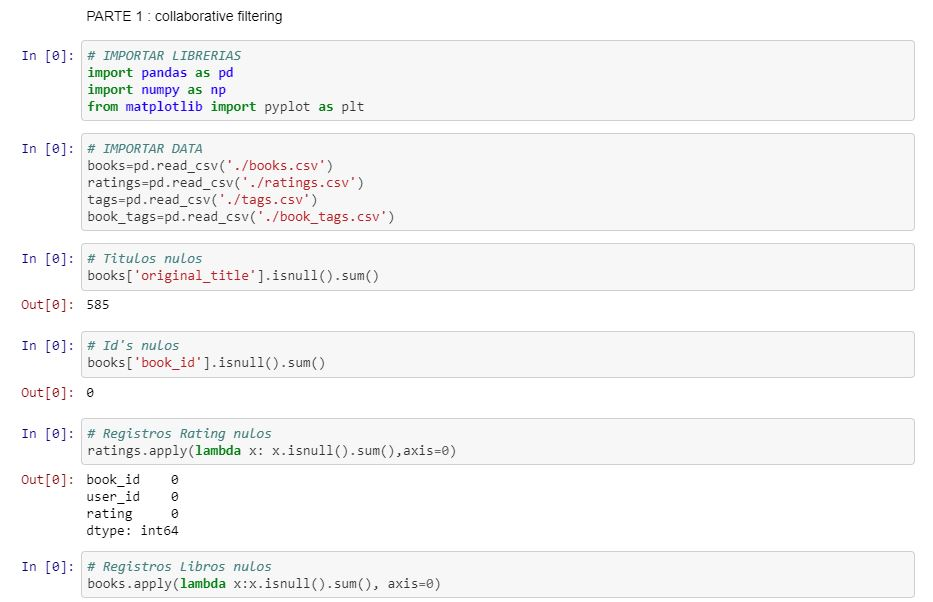
\includegraphics[width=18cm, height=8cm]{./Imagenes/traba1.jpg}
\end{center}


\begin{center}
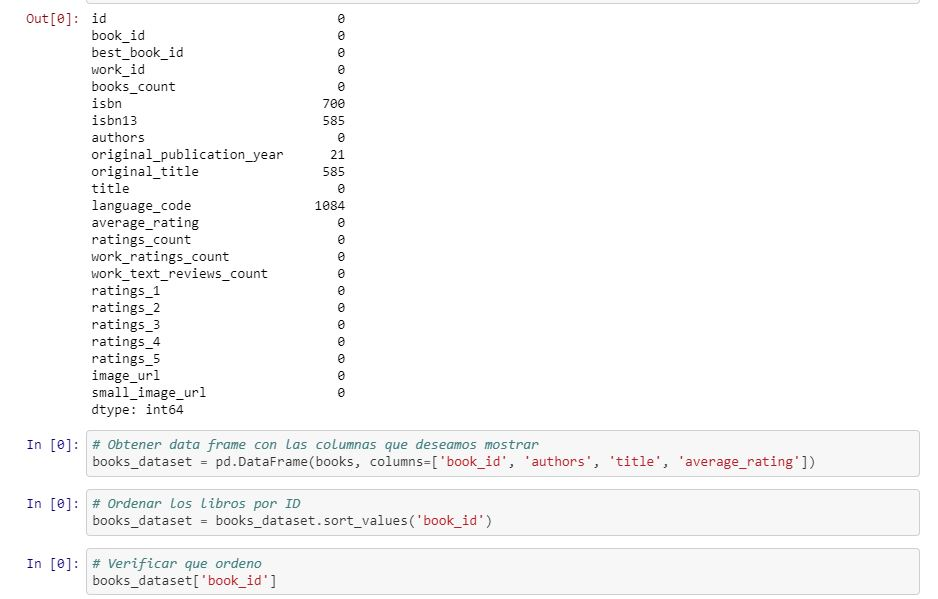
\includegraphics[width=18cm, height=8cm]{./Imagenes/traba2.jpg}
\end{center}


\begin{center}
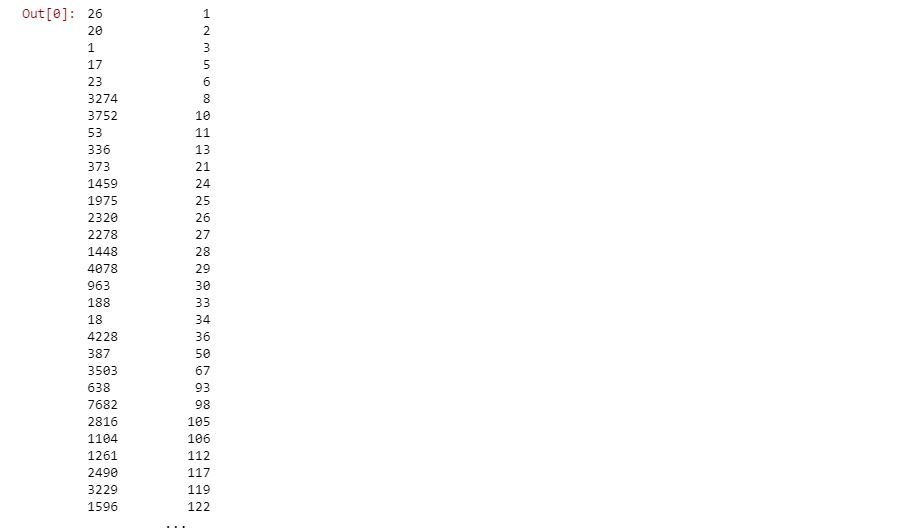
\includegraphics[width=14cm, height=10cm]{./Imagenes/traba3.jpg}
\end{center}


\end{center}


\begin{center}
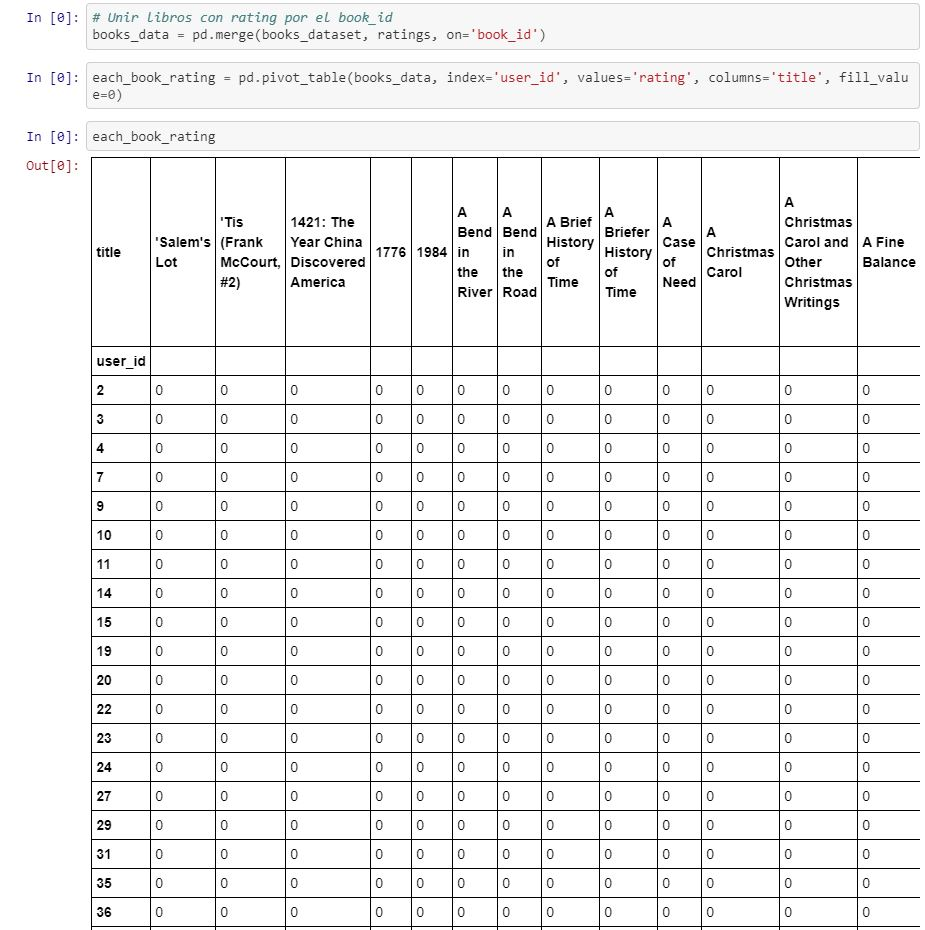
\includegraphics[width=18cm, height=14cm]{./Imagenes/traba5.jpg}
\end{center}

\begin{center}
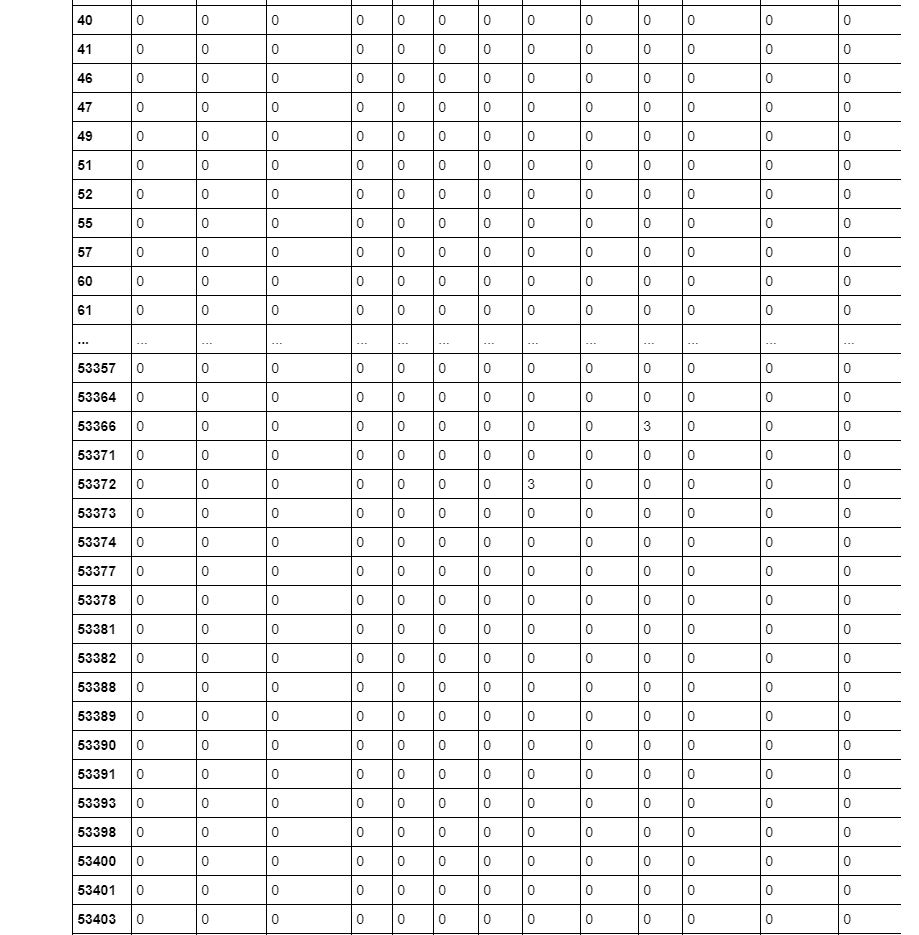
\includegraphics[width=18cm, height=8cm]{./Imagenes/traba6.jpg}
\end{center}


\begin{center}
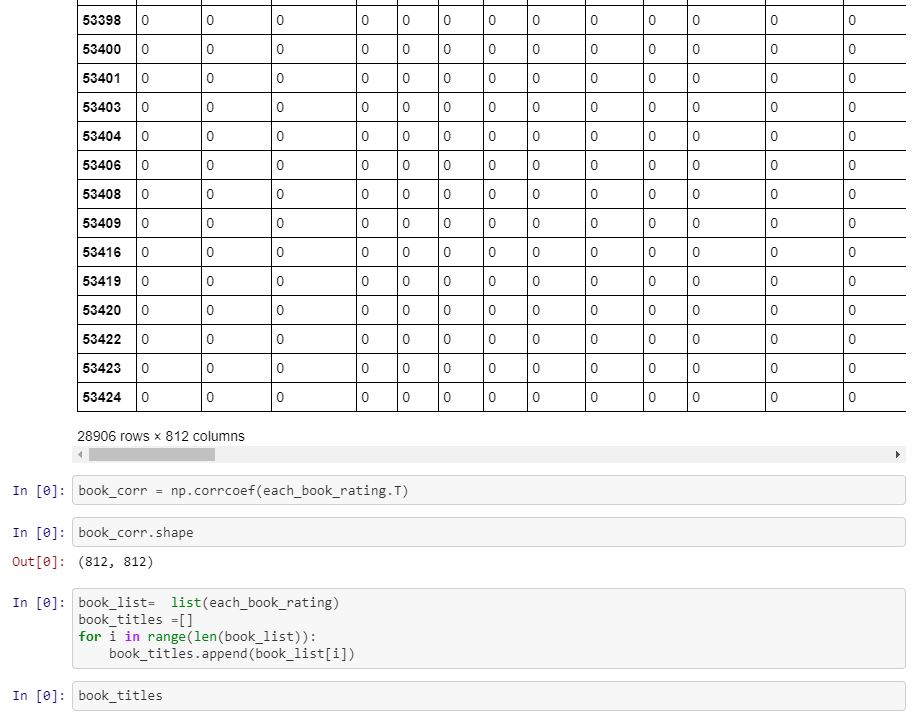
\includegraphics[width=18cm, height=8cm]{./Imagenes/traba7.jpg}
\end{center}


\begin{center}
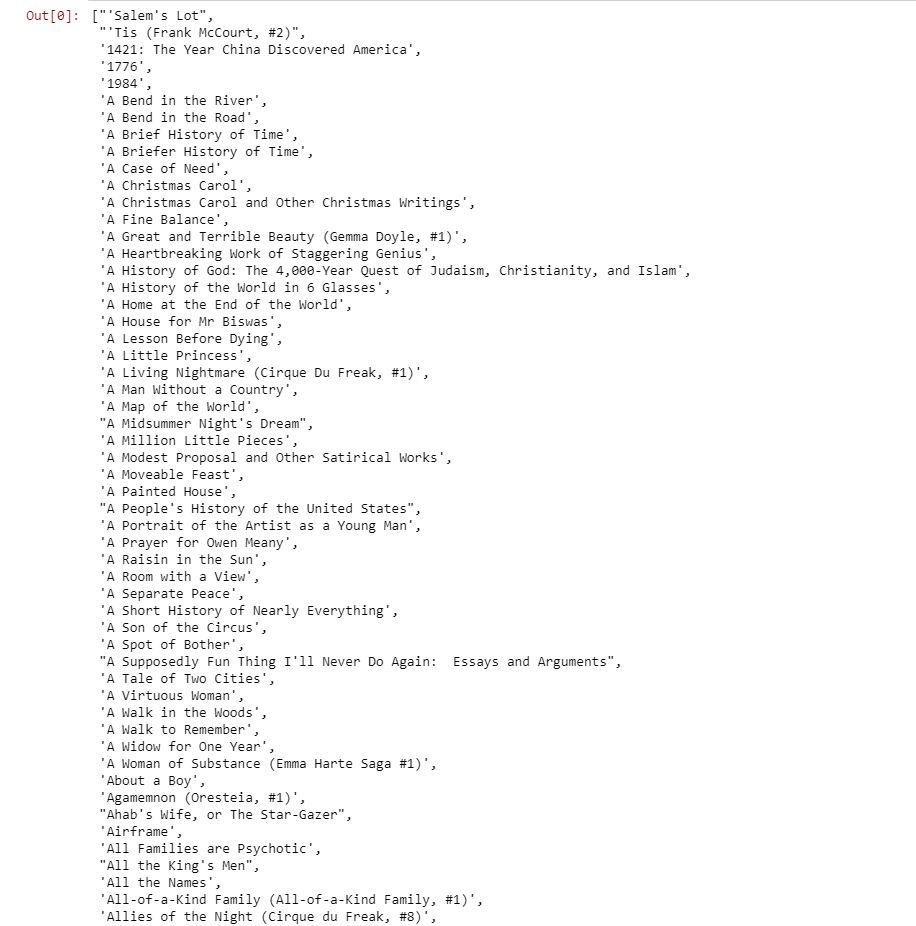
\includegraphics[width=14cm, height=10cm]{./Imagenes/traba8.jpg}
\end{center}


\begin{center}
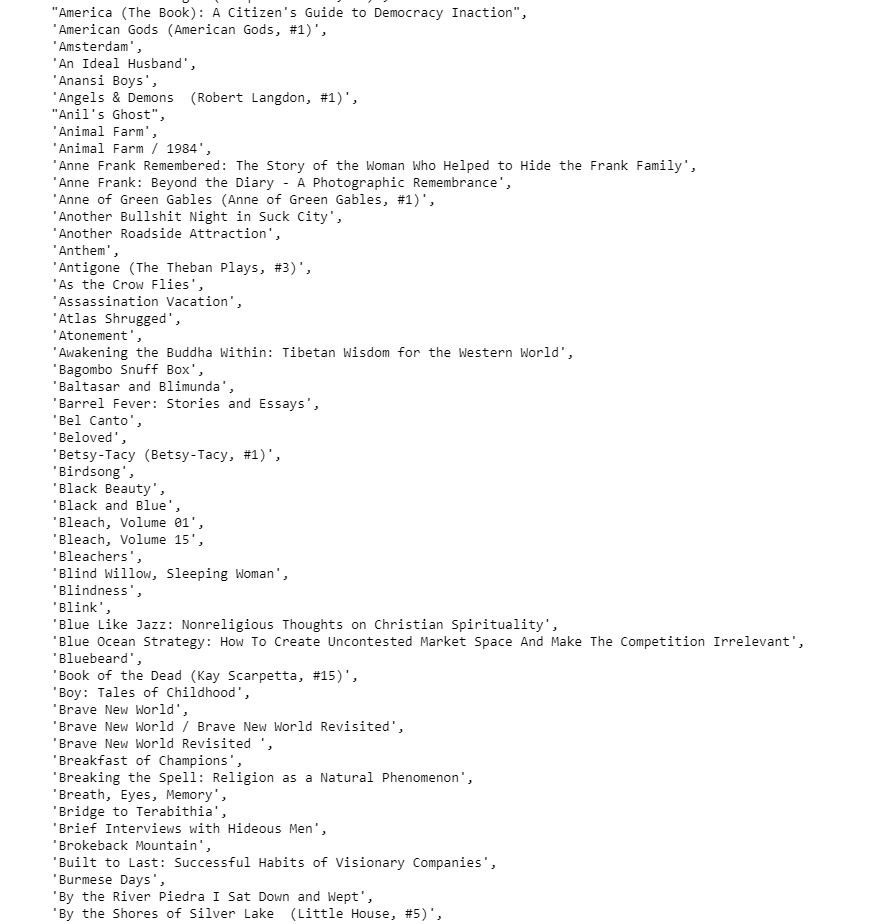
\includegraphics[width=14cm, height=12cm]{./Imagenes/traba9.jpg}
\end{center}


\begin{center}
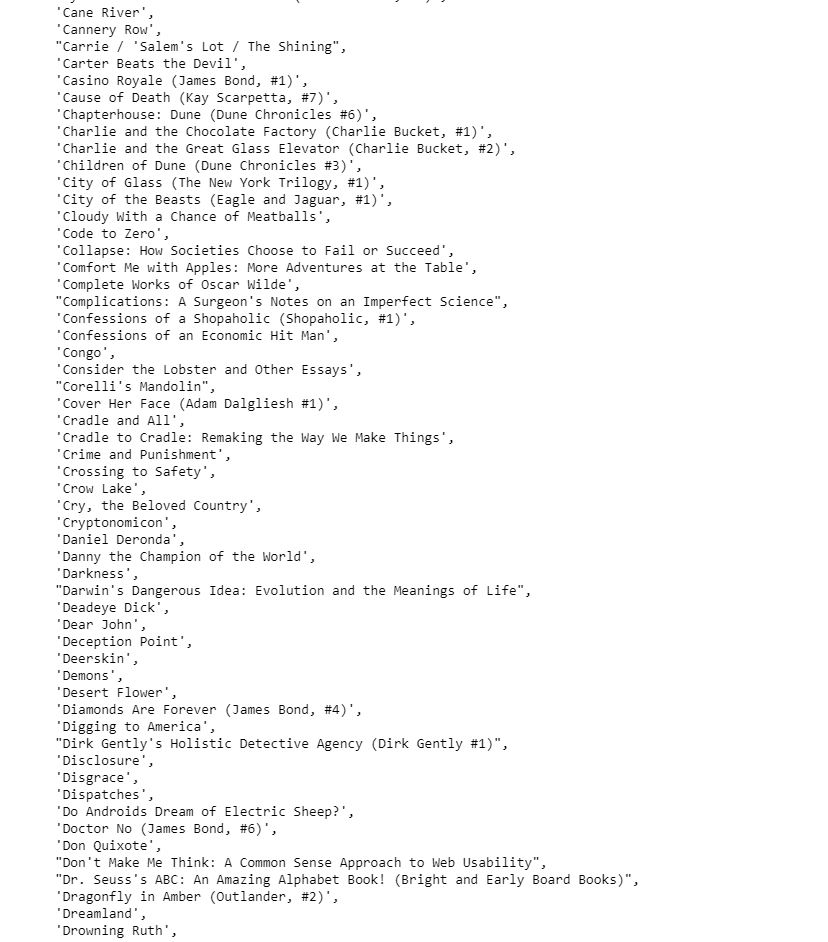
\includegraphics[width=18cm, height=14cm]{./Imagenes/traba10.jpg}
\end{center}

\begin{center}
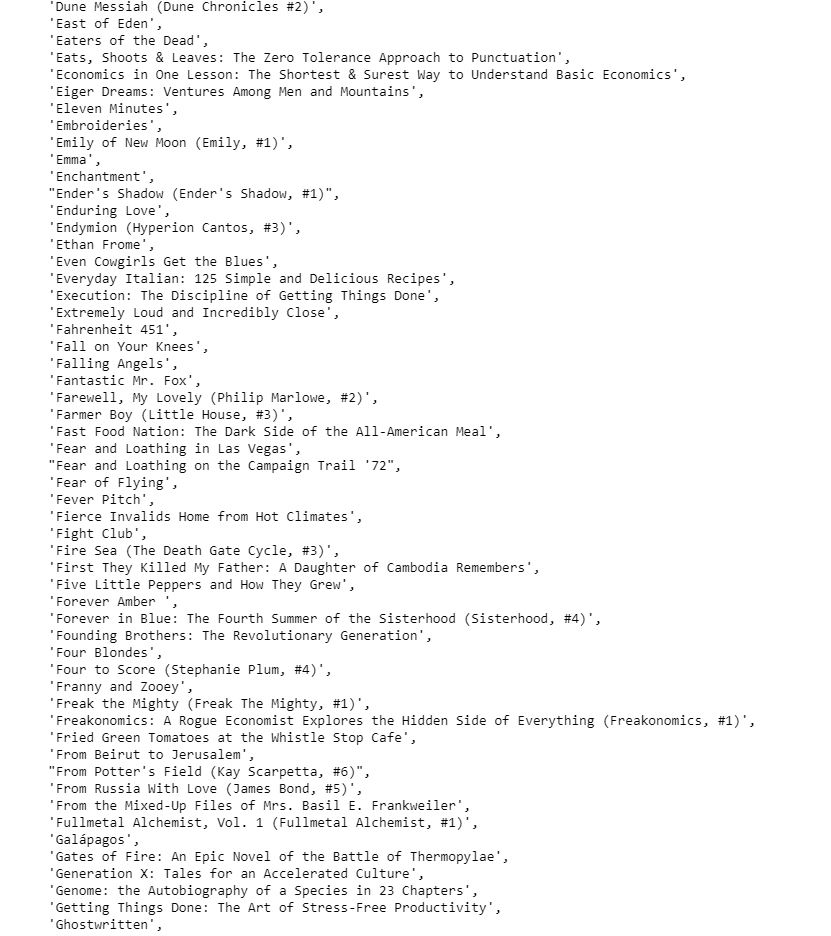
\includegraphics[width=18cm, height=8cm]{./Imagenes/traba11.jpg}
\end{center}


\begin{center}
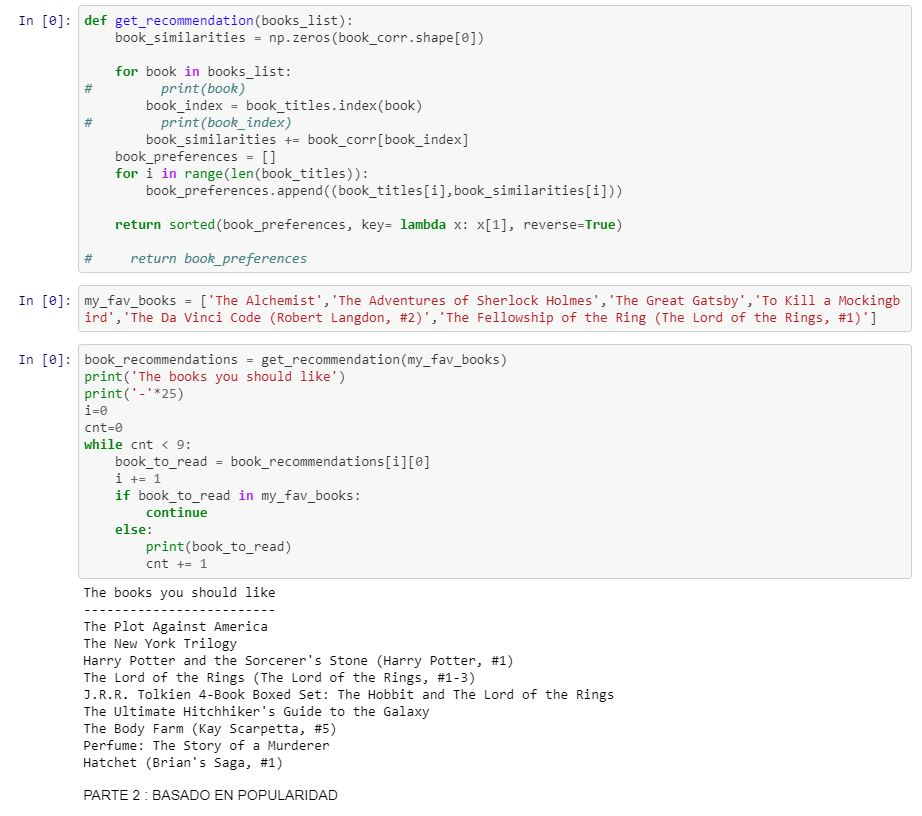
\includegraphics[width=18cm, height=8cm]{./Imagenes/traba12.jpg}
\end{center}


\begin{center}
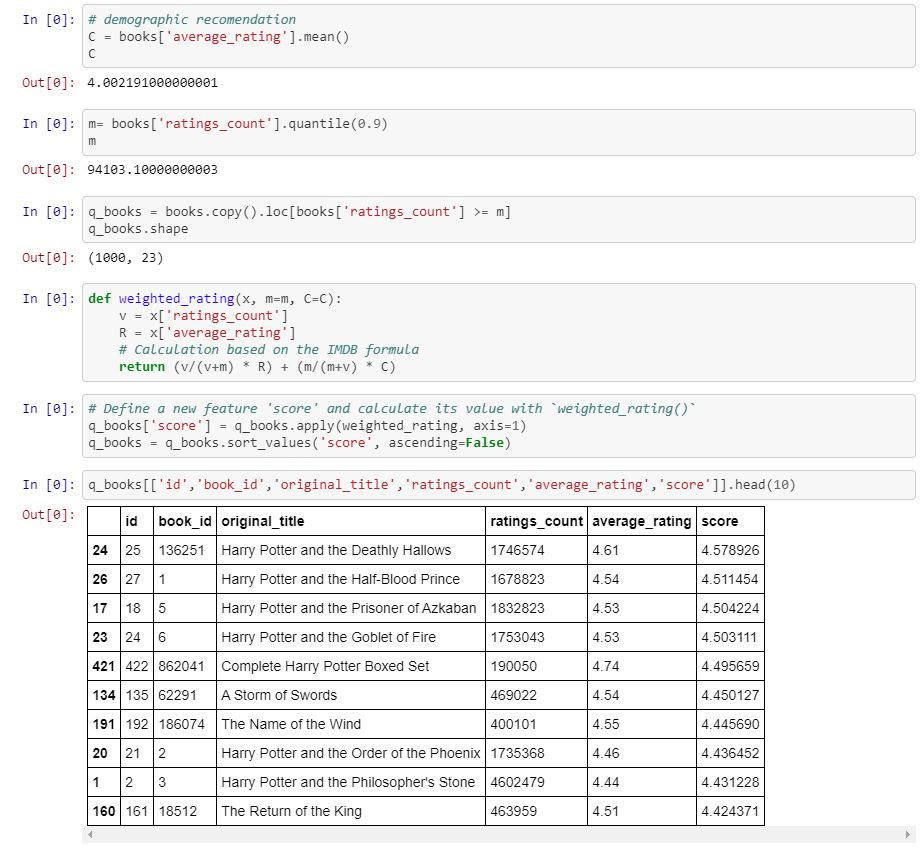
\includegraphics[width=14cm, height=10cm]{./Imagenes/traba13.jpg}
\end{center}


\begin{center}
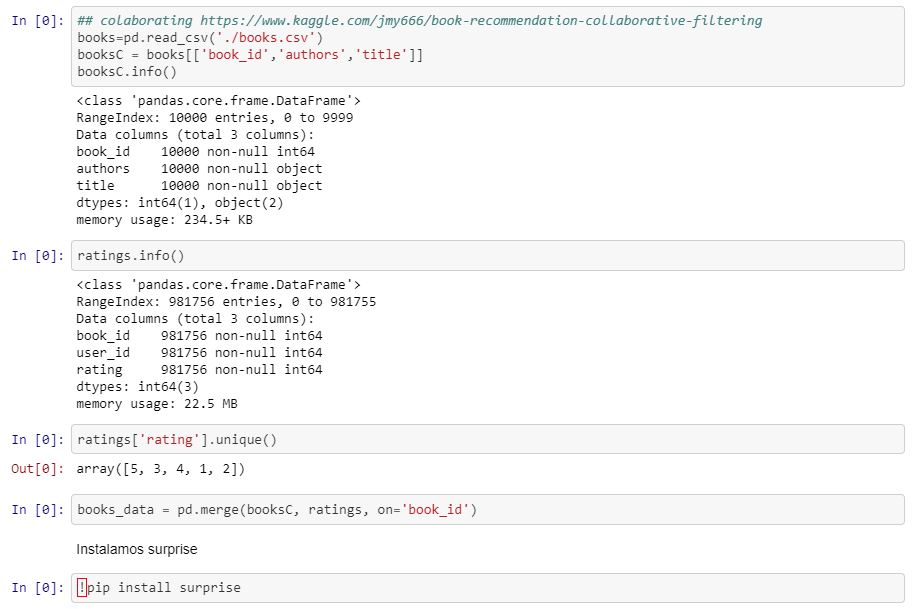
\includegraphics[width=14cm, height=12cm]{./Imagenes/traba14.jpg}
\end{center}


\begin{center}
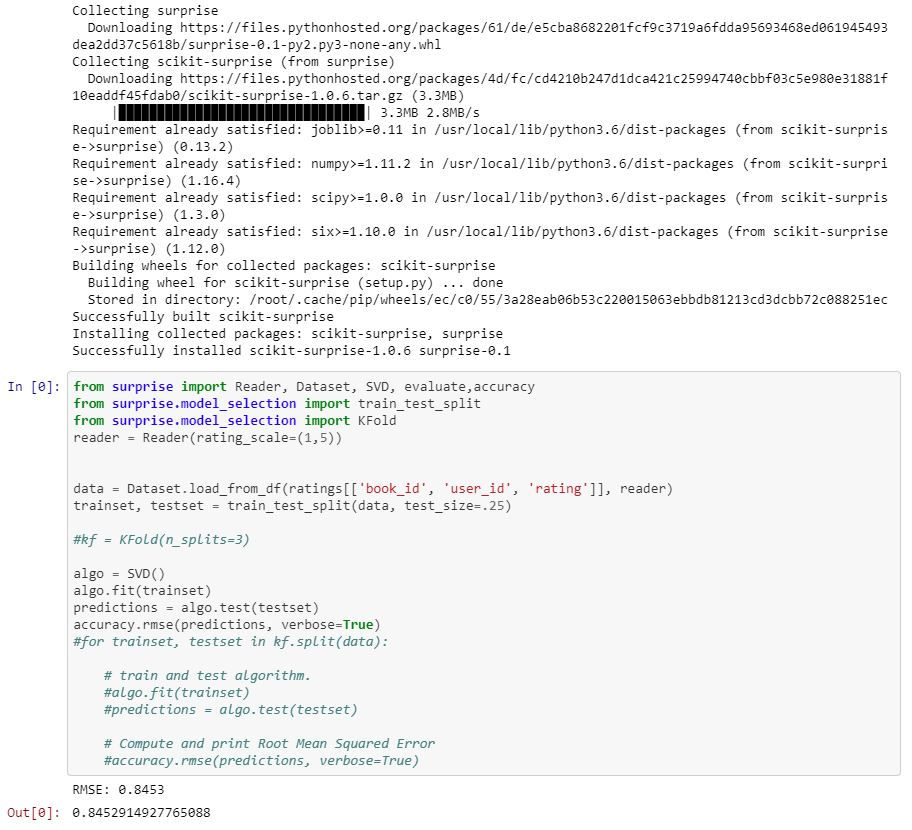
\includegraphics[width=18cm, height=14cm]{./Imagenes/traba15.jpg}
\end{center}

\begin{center}
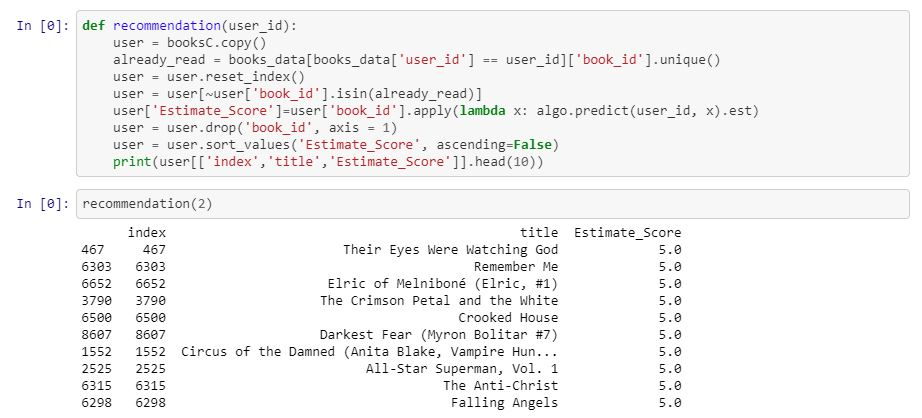
\includegraphics[width=18cm, height=14cm]{./Imagenes/traba16.jpg}
\end{center}